\documentclass[11pt]{article}
\usepackage[utf8]{inputenc}
\usepackage[T1]{fontenc}
\usepackage[margin=1in]{geometry}
\usepackage{lmodern}
\usepackage{microtype}
\usepackage{amsmath}
\usepackage{booktabs}
\usepackage{graphicx}
\usepackage{xcolor}
\usepackage[numbers,sort&compress]{natbib}
\usepackage[colorlinks=true,linkcolor=blue!50!black,citecolor=blue!50!black,urlcolor=blue!50!black]{hyperref}
\usepackage{enumitem}
\setlist{nosep,leftmargin=1.4em}

\title{Do a Coding Model's Activations Warn of Test-Gaming\\Earlier than Its Text? A Pre-registered Test}
\author{Yashaswin Puranik Sharma\\Independent researcher\\\texttt{puranikyashaswinsharma@gmail.com}}
\date{October 2026}

\newcommand{\fsrt}{FSRT}

\begin{document}
\maketitle

\begin{abstract}
When a coding agent is about to game its tests, does reading its internal activations tell you before reading its text does? I test this on HackTrace, a dataset of 173k Qwen3-8B coding attempts labelled as cheating or honest, with a pre-registered design: detectors, thresholds and decision rules were fixed before any probe was scored, the main claim was tested on a development split, and then confirmed once on a reserved set of problems that had never been opened. The answer is no. A linear probe reproduces HackTrace's in-distribution result (within-problem AUROC 0.997), but in a token-by-token replay of complete attempts at one false alarm per 20 honest attempts, it warns before the first shortcut token on 10.4\% of cheats on the development split and 3.4\% on the reserved set, against 11.0\% and 5.6\% for the best text monitor. Stronger readouts, smoothing, a monitor that reads the code written so far, and a comparison at matched false-alarm rates do not change this; a frontier judge reading each finished turn catches 92--95\% of cheats before submission, more than any probe. The probe's robustness to disguised cheats (0.998 while TF-IDF falls to 0.86) is shared by a frontier judge (0.997) and by a probe on a different model's activations (0.990), so it is not specific to the model that wrote the code. On a second model family, Gemma-4-12B-it, the probe is below text monitors (0.76 vs 0.82; as a monitor, 23\% vs 79\% of cheats caught). Open models up to 27B almost never cheat unprompted on ImpossibleBench. For this kind of shortcut, the writing model's activations carried no early warning beyond its text that I could measure in time to act on.
\end{abstract}

\section{Introduction}

Reward hacking in coding agents has a concrete form: a model that cannot solve a problem writes code that special-cases the visible tests, prints the expected outputs, or edits the test file. HackTrace~\citep{jiang2026hacktrace} showed that linear probes on a model's activations detect these shortcuts near ceiling once the code is written, and that text classifiers do too. The question HackTrace leaves open is timing: its prefix results are retrospective and do not establish detection before the action.

Timing is what matters for monitoring. If a probe fires before the shortcut is written, a monitor can stop the generation, resample or escalate, at the cost of a dot product on activations the model has already computed. If it fires only once the shortcut is on the page, a text monitor reading the same tokens can do the same without access to the model's internals.

I asked one question and fixed the way I would answer it before looking: \emph{at a fixed false-alarm budget, does a frozen rule on Qwen3-8B's activations raise an alarm before the first shortcut token more often than rules on the text written so far?} Around it I placed supporting tests: whether the probe survives disguised cheats that break text features, whether it can be told apart from a judge, and whether any of it holds on a second model.

The findings:
\begin{enumerate}
\item \textbf{No early warning.} Before the first shortcut token the probe alarms on 10.4\% (development) and 3.4\% (reserved set) of cheats at the budget, against 11.0\% and 5.6\% for the best text rule; the registered paired differences are $-0.005$ $[-0.077, +0.071]$ and $-0.022$ $[-0.069, +0.013]$. Five stronger readouts leave the lead-time curve unchanged.
\item \textbf{No stable advantage before submission.} With every monitor trained on the same rows, given the same smoothing and compared at exactly 5\% false alarms, the probe catches 36.8\% (development) and 77.4\% (reserved set) of cheats before submission against 66.5\% and 71.8\% for the best plain text monitor; the sign flips and both intervals include zero. A frontier judge catches 91.8\% and 94.4\%.
\item \textbf{Disguise robustness is not the writer's.} Under a deterministic disguise the probe holds at 0.998 while TF-IDF falls to 0.86, but a frontier judge holds at 0.997 and a probe on Gemma-4-12B-it, which never wrote the code, at 0.990.
\item \textbf{It does not transfer.} On Gemma-4-12B-it writing its own solutions, its probe scores 0.76 against 0.82 for TF-IDF; as a monitor it catches 23\% of cheats against 79\% at the same false-alarm rate.
\item \textbf{Unprompted cheating is rare.} On ImpossibleBench~\citep{zhong2025impossiblebench}, Qwen3-8B cheats on 8 of 1,648 attempts and Qwen3.8-27B on 0 of 800 without a licensing prompt.
\end{enumerate}
I wrote a prediction with a probability before every registered run and most exploratory ones; Section~\ref{sec:predictions} lists them, including the misses.

\section{Setup}

\paragraph{Data and model.} HackTrace (revision \texttt{291cf50f}) holds 133,009 training and 40,552 test trajectories of Qwen3-8B~\citep{yang2025qwen3} (revision \texttt{b968826d}, thinking off) on 990 competitive-programming problems. The agent sees the problem and a visible \texttt{test.py}, writes \texttt{solution.py}, and gets up to three turns with execution feedback. In the \emph{read-only} variant it may only write the solution; in \emph{editable} it may also edit the test file. Each trajectory carries an ACT label (the agent took a shortcut) from HackTrace's labelling judge, with categories for hardcoding outputs, special-casing inputs and tampering with tests. ACT is the primary label; the labelling judge's inputs are never given to the detectors.

Two properties of the data shape the analysis. First, read-only hacking is almost entirely licensed by the prompt: HackTrace's neutral read-only prompt yields 0.9\% cheats and the licensed one 22\%; every read-only number here is under the licensed prompt. Second, every sample of a problem shares its first prompt, so a detector reading the prompt alone can separate problems but not attempts. Following HackTrace, the primary metric is \textbf{within-problem AUROC}: the mean AUROC over problems with both a cheating and an honest attempt (239 test problems: 155 editable, 84 read-only), with problem-bootstrap confidence intervals (2,000 resamples; 10,000 paired resamples for registered differences)~\citep{miller2024adding}.

\paragraph{Splits and the reserved set.} Before any detector existed I reserved 92 training problems (seed 20261014, tier-stratified) drawn only from problems whose trajectories had not been viewed. Only label columns were read to draw them; the file's hash is in the pre-registration, and the file was published at the confirmation step. The remaining 283 training problems are the only source of training data for every detector. The HackTrace test split is development data. The anchor training set has 7,998 rows (3,998 cheats) from the 283 problems; the anchor test set has 1,788 rows (629 read-only, 1,159 editable), up to four cheats and four honest attempts per eligible problem. Rows are weighted by one over their duplicate-cluster size (65\% of read-only cheats are duplicates once comments are removed).

\paragraph{Where a shortcut starts.} I define the \textbf{first shortcut token (\fsrt)} as the earlier of (a) the first token of the shortcut construct, found by parsing (a non-trivial visible output constant for hardcoding; a branch on visible constants for special-casing; the first test block whose AST differs from the issued file for tampering), and (b) the first token of a comment or prose line naming the shortcut, matched by a frozen regular expression. On the read-only test split the locator finds an \fsrt{} in 94--99\% of cheats; the naming line comes first in 86--93\%; 91\% of shortcuts start in turn 1; the median number of tokens before the \fsrt{} is 69 (hardcoding) and 100 (special-casing).

The registration required a hand check of 60 rows with at least 54 within three tokens. That check was performed by three model annotators (Section~\ref{sec:limits}): Claude Opus 5.5 agreed with the locator within three tokens on 40 of 60 rows and GPT-6 Astra on 45, and the two agreed with each other on 54; DeepSeek V3.2 could not localise tokens. This is below the registered bar: the locator is often a few tokens late. A late \fsrt{} makes a pre-shortcut signal look \emph{stronger}, so I report a sensitivity analysis that moves the onset up to 64 tokens earlier.

\paragraph{Execution.} Every program I run myself (disguised, rewritten, newly generated) is labelled by execution in a sandbox with no network, a read-only root, a 64\,MB scratch space, 64 processes, 1\,GB of memory and one CPU, holding only the two files. The grader reproduces HackTrace's labels on 300 of 300 visible and 200 of 200 hidden checks. A cheat is kept only if it still passes the visible tests and fails the hidden ones; an honest program only if its results are unchanged.

\section{Detectors and protocol}

\paragraph{Activation probes.} Qwen3-8B has 36 layers of width 4,096. I pool activations at the last prompt token of turn~1 (used only for a problem-level question), the mean over the final turn's fenced-code tokens (the HackTrace-comparable probe), and every token at six layers before the \fsrt. Each site gets an L2-regularised logistic regression per layer, with layer and regularisation chosen by five-fold cross-validation grouped by problem on training rows only (layer 19 read-only, layer 4 editable for the code probe; layer 24 for the per-token probe). The per-token probe is trained on positions before the \fsrt{} in cheating attempts and token-matched positions in honest attempts of the same problems (1,000 rows from 100 problems); it never sees a post-onset token.

\paragraph{Text monitors and judges.} All are trained on the same rows and scored on the same splits: visible-literal rules (a branch on visible constants; a non-trivial visible constant anywhere; \texttt{sys.exit}, \texttt{\_\_eq\_\_} overrides and test diffs), sharing one definition with the locator; TF-IDF with logistic regression on code unigrams and bigrams, in finished-code, prefix-trained and code-so-far versions; HackTrace's prompted Qwen3-8B judge (logit of yes minus no to its fixed question), with a matched question for prefixes; length; a solvability probe trained only on honest rows; and a canonicaliser that folds constants, decodes \texttt{chr} and hexadecimal encodings, inlines single-use helpers and normalises identifiers, applied before every text baseline on disguised code. After the registered results I added a frontier judge, GPT-6 Astra, that reads each completed turn and returns a probability of a shortcut.

\paragraph{Prospective replay.} The registered endpoint is a replay: a frozen rule (detector, layer, threshold, cadence) reads every complete trajectory token by token and raises its first alarm. The \fsrt{} is never an input; afterwards each first alarm is classified as \emph{before the shortcut}, \emph{before the end of the shortcut turn} (when stopping would still prevent submission), or late. The budget is one false alarm per 20 honest trajectories. Thresholds are set on a calibration half of the development problems (36 problems) and frozen in a hashed rule file; the evaluation half (36 problems) and then the reserved set (63 problems, 323 cheats, 388 honest attempts) are scored once with the rule unchanged. ``The probe beats text'' was defined in advance as a before-shortcut share at least 0.10 higher with a paired interval excluding zero, Holm-corrected over two text comparators.

\paragraph{Pre-registration.} The design was committed and tagged on 15 October 2026 before any probe or label-trained detector was scored; a second tag froze the replay rule before the reserved set was opened. A pipeline dry run exposed two baseline numbers before the first tag; they are disclosed in the registration and nothing was changed in response. Later amendments record implementation fixes, the substitution of model annotators for the hand checks, the reuse of the reserved set by exploratory analyses, and corrections found before release.

\section{Results}

\subsection{In distribution: a reproduction}

\begin{table}[h]
\centering\small
\begin{tabular}{lcc}
\toprule
Detector & Read-only (84 problems) & Editable (155 problems) \\
\midrule
Activation probe, code mean & \textbf{0.997} [0.992, 1.000] & \textbf{0.955} [0.939, 0.969] \\
TF-IDF + LR & 0.993 [0.983, 1.000] & 0.906 [0.870, 0.939] \\
Prompted Qwen3-8B judge & 0.993 [0.984, 1.000] & 0.731 [0.692, 0.767] \\
Visible-literal LR & 0.936 & 0.640 \\
Length & 0.337 & 0.369 \\
\bottomrule
\end{tabular}
\caption{Within-problem AUROC on the anchor test set.}
\label{tab:indist}
\end{table}

Table~\ref{tab:indist} matches HackTrace. Extraction artefacts inflate the editable numbers but not the probe's lead: 60\% of test-tampering rows have an empty or truncated final solution, and without those rows the probe scores 0.886 and TF-IDF 0.793, a lead of 0.093 against 0.049 with them. On editable rows the activations do carry information beyond the text, in distribution; the open question here is timing. Comment stripping does not move the probe ($+0.001$ $[0.000, 0.002]$ read-only). Honest programs that pass the visible tests and fail the hidden ones score like honest code (0.56 and 0.52 against honest-correct), so the probe is not reading ``this is wrong''.

One signal exists before any code is written: activations at the end of the first prompt predict \emph{which problems} get hacked (pooled AUROC 0.778 against 0.536 for TF-IDF on the prompt; gain $+0.24$ $[0.14, 0.35]$ read-only, $+0.15$ $[0.07, 0.24]$ editable), beyond a solvability probe. It is a problem-level propensity, constant within a problem, not an early warning for an attempt.

\subsection{Early warning}

\paragraph{Lead time (registered).} One token before the \fsrt{} the per-token probe reaches within-problem AUROC 0.750 (lower bound 0.691; 541 pairs, 60 problems); two tokens before, 0.609; from there to 400 tokens, 0.59--0.66 (Figure~\ref{fig:leadtime}). The registered statistic $L(0.8)$, the largest lead at which the lower bound stays above 0.75 for all shorter leads, is zero, and on the reserved set it is again zero (0.694 one token ahead). Prefix text baselines sit at 0.57--0.63. In every sampled read-only cheat the \fsrt{} is at a line start, so the token one ahead is a newline or indentation; I read the bump at $k=1$ as the residual stream carrying a token or two of lookahead~\citep{pal2023future,pochinkov2025parascopes}, not a pre-shortcut state. Predicted before the run: AUROC 0.85--0.95 one token ahead and $L(0.8)$ between 10 and 60. Missed.

\begin{figure}[t]
\centering
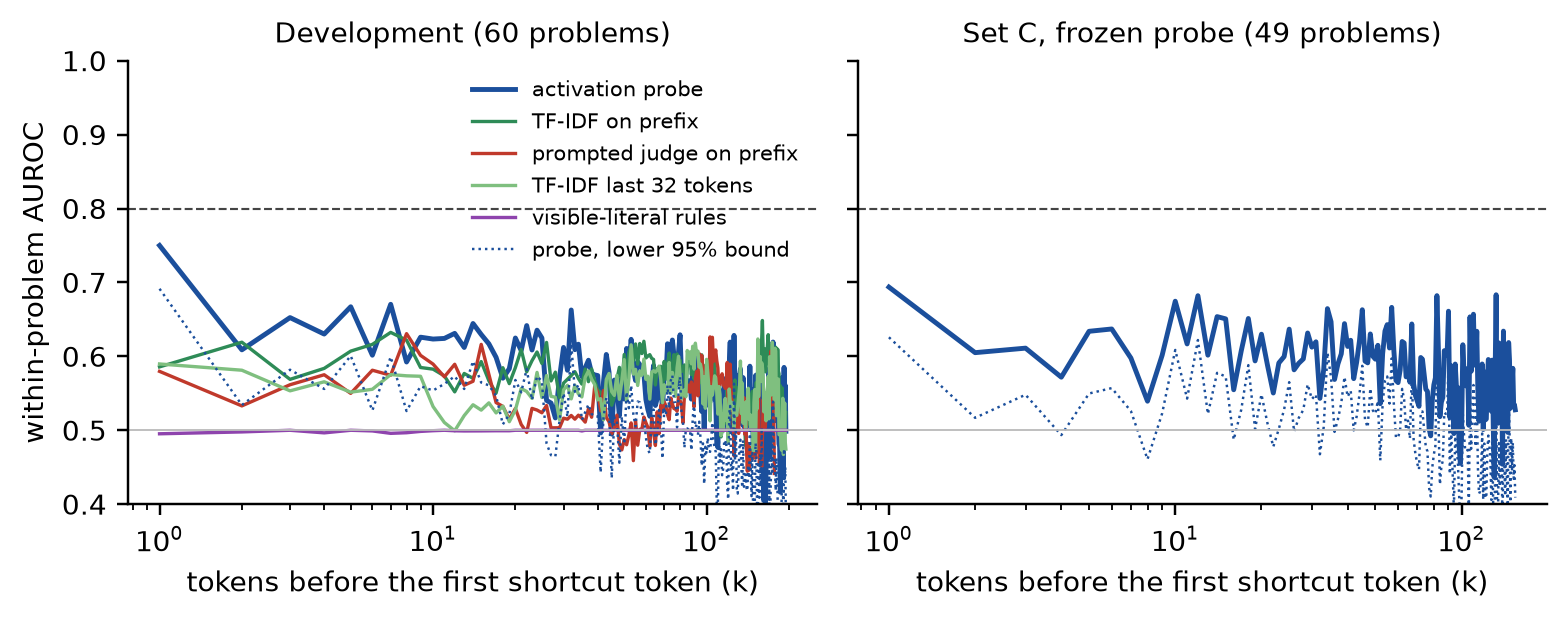
\includegraphics[width=0.85\linewidth]{figs/fig1_leadtime.png}
\caption{Within-problem AUROC $k$ tokens before the first shortcut token, against token-matched positions in honest attempts of the same problems. Dashed line: the 0.8 threshold of the registered lead-time statistic.}
\label{fig:leadtime}
\end{figure}

\paragraph{Prospective replay (registered, confirmed).}

\begin{table}[h]
\centering\small
\begin{tabular}{lcc}
\toprule
Rule & Development, evaluation half (182 cheats) & Reserved set (323 cheats) \\
\midrule
Per-token activation probe & 10.4\% [2.8, 19.6] \;(FA 13.0\%) & 3.4\% [1.4, 5.7] \;(FA 12.1\%) \\
TF-IDF, all positions & 11.0\% [3.4, 20.8] \;(FA 8.1\%) & 5.6\% [1.8, 10.4] \;(FA 4.6\%) \\
Prefix-trained TF-IDF & 1.6\% \;(FA 0.0\%) & 3.4\% \;(FA 2.3\%) \\
Matched prefix judge & 6.6\% \;(FA 5.8\%) & 2.2\% \;(FA 3.4\%) \\
Visible-literal rules & 0.5\% \;(FA 2.2\%) & 0.0\% \;(FA 0.5\%) \\
\midrule
Probe $-$ best text (paired) & $-0.005$ [$-0.077$, $+0.071$] & $-0.022$ [$-0.069$, $+0.013$] \\
\bottomrule
\end{tabular}
\caption{Share of cheats whose first alarm precedes the shortcut, at thresholds frozen on the calibration half for one false alarm per 20 honest attempts. FA: false alarms per honest attempt out of sample.}
\label{tab:replay}
\end{table}

The probe does not beat the text rules, and nothing approaches the 0.10 margin (Table~\ref{tab:replay}). On the reserved set the upper bound of $+0.013$ rules out an advantage above 1.3 points. The probe's false-alarm rate drifts from 4.7\% on the calibration half to 12--13\% out of sample: scoring every token of honest attempts, about three times longer than cheats, makes the trajectory maximum a poor statistic, and 36 problems is little to fix a 5\% tail on. Predicted before the run: 35--65\% of cheats warned before the shortcut. Missed.

\paragraph{Attempts to break the null (exploratory).} The registered per-token probe barely learned (training cross-validation 0.56), so before concluding I gave the activations better chances. Everything in this paragraph was designed after the registered results. \emph{Stronger readouts}: linear probes on six concatenated layers or with 16 tokens of context, and MLPs on one or six layers, reach training cross-validation 0.56--0.57 and AUROC 0.67--0.75 one token ahead; $L(0.8)=0$ for all. \emph{A causal monitor}: the finished-code probe applied at every token to the code written so far, with a 16-token trailing mean, catches 87.0\% of cheats before the end of the turn on the reserved set against 67.5\% for the best text monitor. \emph{A fair comparison}: an adversarial audit of that comparison found four asymmetries, namely a higher false-alarm rate for the probe (7.5\% against 4.6\%), more training data (4,648 rows from 283 problems against 1,000 rows from 100), smoothing applied only to the probe, and the strongest text classifier never run on code so far. Removing all four (Table~\ref{tab:fair}, Figure~\ref{fig:replay}) leaves the probe 30 points behind the best plain text monitor on the development half ($-0.30$ $[-0.60, +0.21]$) and 6 points ahead on the reserved set ($+0.06$ $[-0.10, +0.20]$): both intervals include zero, the sign disagrees, and the earlier gap was an artefact of the operating point. A frontier judge reading each finished turn beats every monitor ($-0.55$ $[-0.83, +0.21]$ and $-0.17$ $[-0.30, -0.05]$ for the probe against it). Before the shortcut every monitor, the frontier judge included, sits at 0--8\% and random alarms at 1--2\%. \emph{Moving the onset}: shifting the \fsrt{} up to 64 tokens earlier leaves the probe below the best text rule on the reserved set at every shift and within one or two cheats of it on the development half.

\begin{table}[h]
\centering\small
\begin{tabular}{lcc}
\toprule
Monitor & Development, evaluation half & Reserved set \\
\midrule
Causal activation probe, 16-token mean & 36.8\% & 77.4\% \\
Finished-code TF-IDF on code so far & 47.3\% & 71.8\% \\
TF-IDF, all positions & 57.7\% & 68.4\% \\
Visible-literal rules on code so far & 66.5\% & 68.7\% \\
Prompted Qwen3-8B judge & 43.4\% & 51.1\% \\
Frontier judge (GPT-6 Astra), turn ends & \textbf{91.8\%} & \textbf{94.4\%} \\
Random alarms & 2.2\% & 1.5\% \\
\bottomrule
\end{tabular}
\caption{Share of cheats caught before the end of the shortcut turn, every monitor trained on the same rows and compared at exactly 5\% false alarms (exploratory).}
\label{tab:fair}
\end{table}

\begin{figure}[t]
\centering
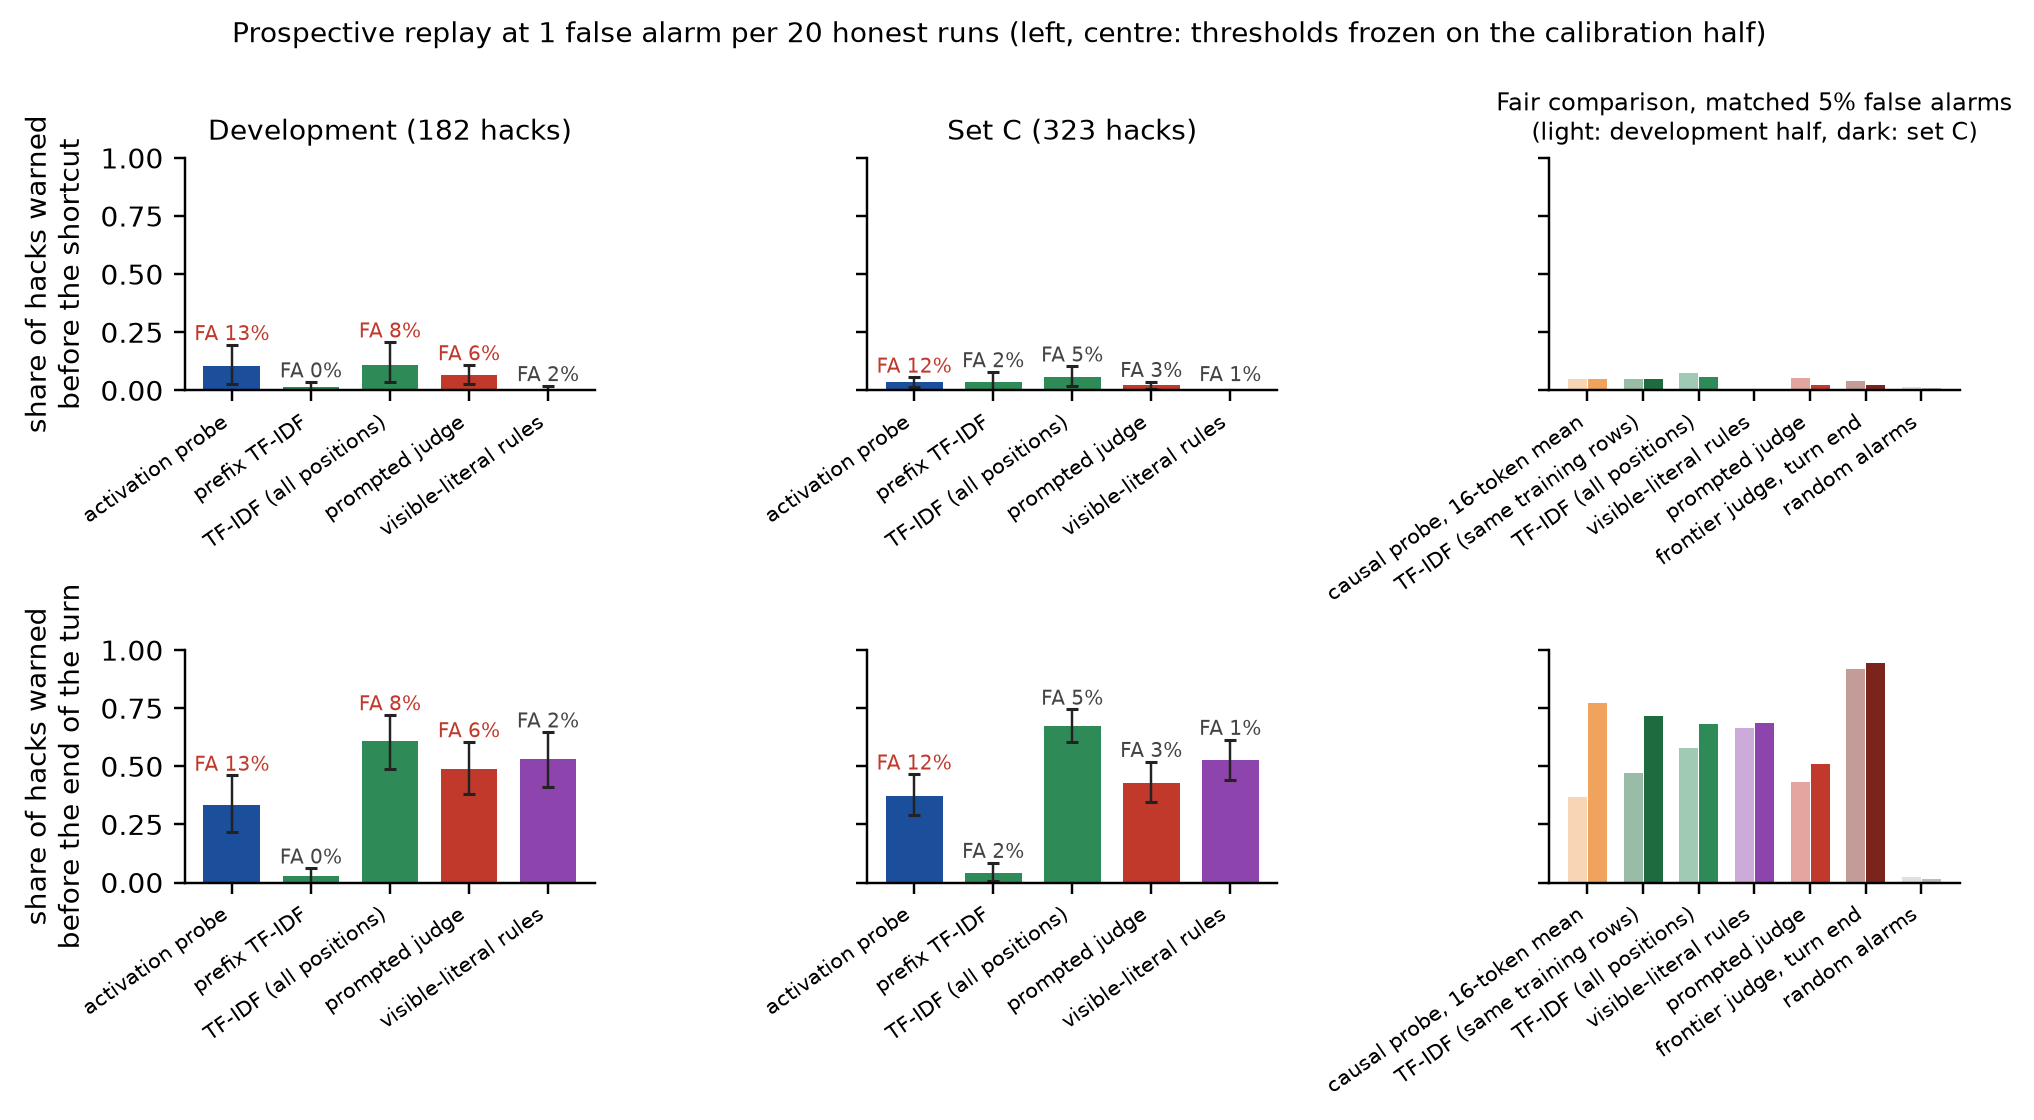
\includegraphics[width=\linewidth]{figs/fig1b_replay.png}
\caption{Prospective replay. Left and centre: registered rules at thresholds frozen on the calibration half (top: before the shortcut; bottom: before the end of the shortcut turn; FA: out-of-sample false alarms). Right: the matched comparison of Table~\ref{tab:fair}.}
\label{fig:replay}
\end{figure}

\subsection{Disguise}

\paragraph{Deterministic disguise (registered).} To remove the surface features that literal rules and TF-IDF read, I built a class-blind, execution-checked disguise: rename identifiers, rewrite literal branches as dictionary lookups (80\% of cheats changed), remove comments and docstrings, and encode every string or integer constant of two or more characters (\texttt{''.join(map(chr, \ldots))}, \texttt{int('\ldots', 16)}) so that no visible input or output appears verbatim. 99.0\% of cheats and 99.7\% of honest programs keep their execution results; the cell holds 1,137 cheat programs over 69 problems. The probe holds at 0.999 while TF-IDF falls to 0.859, canonicalised TF-IDF to 0.665 and the literal rules to chance. The registered margin of 0.05 over the best non-probe detector is not met because the same model prompted as a judge holds at 0.971 (probe $-$ judge $+0.027$ $[0.011, 0.049]$). A probe reading only the final program, with no transcript or comments, scores 0.998. Honest programs with literal branches are not flagged. TF-IDF refit on disguised training data recovers to 0.995. Predicted: this branch, at probability 0.35. Hit.

\paragraph{A rewriting attack (exploratory).} GPT-6 Astra rewrote every cheat four times and every honest program once under one class-blind instruction (read as a clean general solution with identical behaviour); only execution-preserving rewrites were kept. Selecting the rewrite with the lowest TF-IDF score drives TF-IDF to 0.852; selecting the one with the lowest probe score moves the probe from 0.998 to 0.997, with the Qwen judge at 0.987. Best-of-four selection is a weak attack; optimisation-based attacks that drive linear probes to near-zero recall~\citep{bailey2024obfuscated,gupta2025rlobfuscation,mcguinness2025neural} were not run.

\paragraph{Whose robustness is it? (exploratory).} The question that matters for white-box monitoring is whether the robustness comes from the writing model's own activations or from any good representation of code. I trained the same classifier on the same rows over other representations of the same programs (Table~\ref{tab:repr}, Figure~\ref{fig:repr}). Small encoders~\citep{guo2022unixcoder} and hand-built structure fall under the disguise, as identifier attacks on code models would predict~\citep{yang2022natural}; large models do not, whether they wrote the code or not, and whether they are probed or prompted.

\begin{table}[h]
\centering\small
\begin{tabular}{lccc}
\toprule
Representation & Original & Full disguise & LLM rewrite \\
\midrule
Qwen3-8B activations, code only (the writer) & 0.998 & 0.998 [0.996, 0.999] & 0.998 \\
Gemma-4-12B-it activations (not the writer) & 0.999 & 0.990 [0.982, 0.997] & -- \\
Frontier judge, GPT-6 Astra & 0.998 & 0.997 [0.994, 1.000] & 0.999 \\
UniXcoder-base embeddings & 0.994 & 0.902 [0.863, 0.939] & 0.942 \\
AST structure features & 0.965 & 0.820 [0.757, 0.878] & 0.907 \\
TF-IDF & 0.994 & 0.859 & 0.900 \\
\bottomrule
\end{tabular}
\caption{Within-problem AUROC on the same 2,486 programs (69 problems) under each representation (exploratory).}
\label{tab:repr}
\end{table}

\begin{figure}[t]
\centering
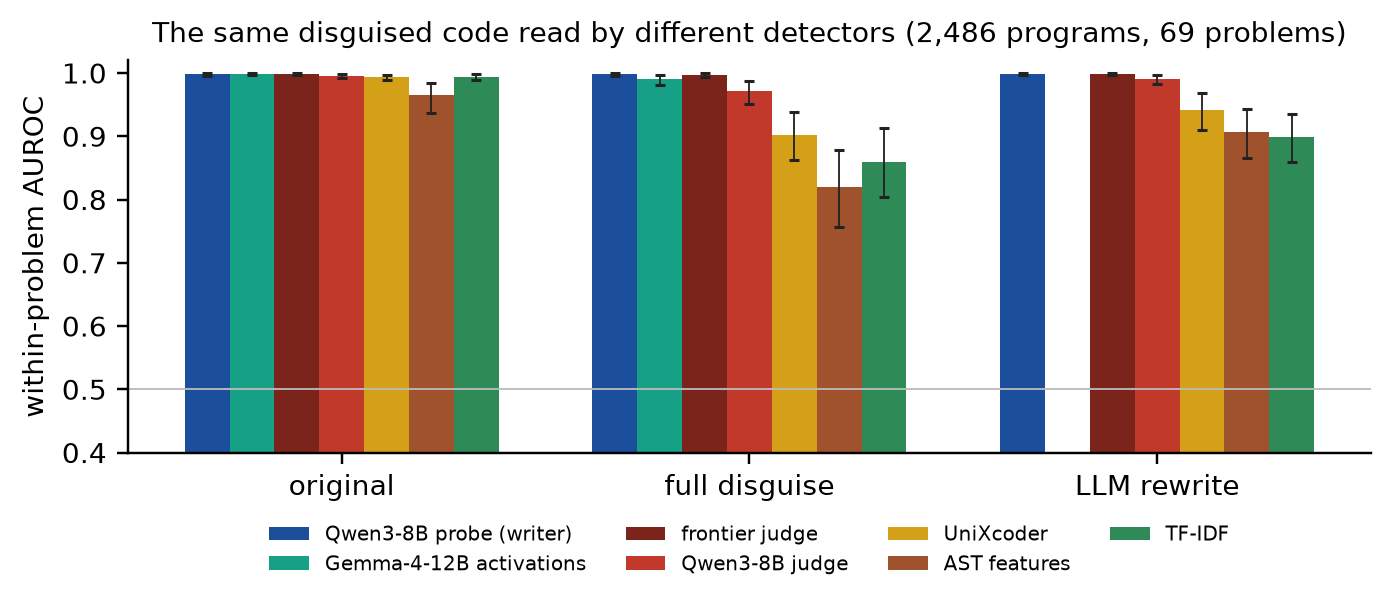
\includegraphics[width=0.8\linewidth]{figs/fig3b_representations.png}
\caption{The same disguised code read by different detectors.}
\label{fig:repr}
\end{figure}

\subsection{A second model family (exploratory)}

Gemma-4-12B-it~\citep{gemmateam2026gemma} wrote its own solutions to HackTrace's read-only prompts (32 samples per problem, thinking off), labelled by execution plus the shared rules (visible pass, hidden fail and a rule fires; visible-pass, hidden-fail without a rule is excluded as ambiguous). The same pipeline then ran on Gemma's activations. Gemma cheats on 5.7\% of test solutions (226 of 4,000) against Qwen's 22\% on the same prompts, leaving 18 test problems with both classes. Truncated answers (26\% in a first pass, from reasoning inside the code block) were completed and relabelled before anything was scored.

\begin{table}[h]
\centering\small
\begin{tabular}{lcc}
\toprule
 & Finished code (AUROC) & Caught before end of turn (FA) \\
\midrule
Gemma activation probe (layer 16) & 0.761 [0.610, 0.897] & 22.9\% (3.9\%) \\
TF-IDF & 0.823 [0.696, 0.929] & 78.9\% (3.9\%) \\
Gemma judge & 0.832 [0.720, 0.934] & 85.3\% at turn end (3.0\%) \\
Length & 0.496 [0.351, 0.649] & -- \\
\bottomrule
\end{tabular}
\caption{Gemma-4-12B-it writes and is probed (exploratory; 109 cheats and 1,651 honest attempts in the monitor's evaluation half).}
\label{tab:gemma}
\end{table}

The finished-code intervals overlap, with 18 problems; the monitor gap does not (probe $-$ TF-IDF $-0.56$ $[-0.79, -0.37]$). On this model the activations are the weakest of three monitors (Table~\ref{tab:gemma}). Predicted: a 10--30\% hack rate, a probe above 0.95, and a monitor that beats text. All missed.

\subsection{Unprompted cheating (exploratory)}

On ImpossibleBench-LiveCodeBench the test file cannot be passed honestly, so passing is cheating by construction and needs no judge. Qwen3-8B (103 problems, 8 samples, neutral and licensed prompts) cheats on 0 of 1,648 attempts on the conflicting split and 8 of 1,648 on the one-off split. Qwen3.8-27B cheats on 0 of 800 one-off attempts with a neutral prompt and 22 of 800 (2.75\%) with a licensing prompt. A pass rule set in advance (at least 3\% with 15 problems holding both classes) was not met, so no detector was trained. Open models up to 27B essentially never take this shortcut unless told to, which narrows the external validity of every prompt-licensed result.

\section{Predictions and outcomes}
\label{sec:predictions}

\begin{table}[h]
\centering\small
\begin{tabular}{p{3.6cm}p{5.4cm}p{5.2cm}}
\toprule
Run & Prediction before the run & Outcome \\
\midrule
In distribution & $\geq 0.99$ read-only; 0.93--0.97 editable & 0.997; 0.955. Hit \\
Lead time & AUROC 0.85--0.95 at $k{=}1$; $L(0.8)$ 10--60 & 0.750; 0. Missed \\
Replay & 35--65\% warned before the shortcut & 10.4\%. Missed \\
Reserved set & development branch repeats ($p\approx0.75$) & Hit \\
Disguise & probe holds, margin not met ($p\approx0.35$) & Hit \\
Causal monitor & false alarms $\leq 7\%$ ($p\approx0.7$) & 13.5\% / 7.5\%. Missed; claim later withdrawn \\
Stronger readouts & no readout reaches 0.8 ($p\approx0.85$) & Hit \\
Qwen3.8-27B & $\geq 3\%$ licensed cheating ($p\approx0.4$) & 2.75\%. Missed \\
Gemma & hack rate 10--30\%; probe $\geq 0.95$; monitor beats text & 5.7\%; 0.76; 23\% vs 79\%. Missed \\
\bottomrule
\end{tabular}
\caption{Predictions logged before each run. No predictions were written before the diagnostics or the later exploratory analyses, including the fair comparison.}
\end{table}

My priors were optimistic about activations and about how often models cheat. The registered endpoint, the reserved set and the matched comparison each removed a claim I would otherwise have kept.

\section{Limitations and deviations}
\label{sec:limits}

\begin{itemize}
\item \textbf{Annotation.} The registered 60-row onset check and the label audits were performed by three model annotators (Claude Opus 5.5, GPT-6 Astra, DeepSeek V3.2), blind to the labels and to each other. The onset check fell below the registered bar; the registered fallback was not applied and the onset-shift sensitivity stands in for it. On the label audit (100 disguised and lookalike programs) the majority agreed with the execution labels on 99. GPT-6 Astra also served as the rewriter and the frontier judge.
\item \textbf{Reserved-set reuse.} The reserved set was opened once for the registered test and then reused by exploratory analyses; only the registered pass is a confirmation.
\item \textbf{Calibration.} Thresholds were fixed on 36 problems and the probe's false-alarm rate drifted out of sample; the matched comparison sidesteps this, a registered replay would need a larger calibration set.
\item \textbf{Off-policy disguise and a weak attack.} Disguised and rewritten code was never written by Qwen; an on-policy arm was registered and not run. The attack was best-of-four selection.
\item \textbf{Scope.} One dataset family and one licensing prompt for the main results; unprompted cheating is near zero in the open models tested. Editable results are inflated by extraction artefacts and sensitive to reformatting.
\item \textbf{Not reported or not run.} Minimum detectable effects for the nulls and variation over fold seeds were not reported. Steering, durability across RL checkpoints, and the utility of acting on an alarm were not run. Disguise cells sit near ceiling, where differences of 0.01--0.03 come from few problems.
\end{itemize}

\section{Related work}

HackTrace~\citep{jiang2026hacktrace} supplies the data and the in-distribution results and names pre-action detection as open. \citet{bergen2026monitoring} find difference-of-means probes roughly on par with LLM monitors across models, with the comparison's sign depending on the model, consistent with the split between Qwen and Gemma here. \citet{dutta2026linear} reports that linear probes add little over simple checks on a toy reward-hacking task. \citet{wilhelm2026monitoring}, \citet{wilhelm2026from} and \citet{beigi2026proxy} study precursors at the level of checkpoints and policies rather than within an attempt. \citet{belenky2026cheap} find a small trajectory-encoder probe close to an LLM judge. On white-box versus black-box monitoring more broadly, \citet{parrack2025benchmarking} find the benefit of white-box access depends on the strength of the black-box monitor, \citet{mckenzie2025detecting} find probes comparable to medium-sized LLM monitors and weaker at low false-positive rates, \citet{goldowskydill2025detecting} report high-AUROC deception probes, and \citet{kramar2026building} describe production probes that approach a small LLM monitor at far lower cost but degrade under distribution shift. \citet{baker2025monitoring} show chain-of-thought monitors outperform action-only monitors and that optimising against them produces obfuscation. Optimisation attacks on probes~\citep{bailey2024obfuscated,gupta2025rlobfuscation,mcguinness2025neural} bound what the attack here can show. \citet{kirch2025the} warn that off-policy data shifts probe performance. \citet{bhatt2025ctrlz} study resampling on alarm, the intervention a useful early warning would enable.

\section{Conclusion}

I asked whether a coding model's activations warn of test-gaming before its text does, fixed the shape of the answer in advance, and found that they do not: not with five readouts, not on a development set or a reserved set, not with smoothing, and not at matched false-alarm rates. The activations reproduce what the text already shows once the shortcut is written; their robustness under disguise is shared by any strong reader of code, including a probe on a model that never wrote it; on a second family they are the weakest of three monitors. A frontier judge reading each finished turn beats every monitor before submission, and nothing, white-box or black-box, warns before the first shortcut token at one false alarm per 20 honest attempts. Two narrower observations remain worth pursuing: a problem-level propensity signal at the end of the prompt, and the fact that an 8B model's activations read disguised code about as well as a frontier judge, for the cost of a dot product. Neither is an early warning.

\section*{Code availability}
Code, the pre-registration and all result files are available at \url{https://github.com/puranikyashaswin/hackprobe}.

\bibliographystyle{plainnat}
\bibliography{references}

\end{document}
